\documentclass[fleqn]{article}
\oddsidemargin 0.0in
\textwidth 6.0in
\thispagestyle{empty}
\usepackage{import}
\usepackage{amsmath}
\usepackage{graphicx}
\usepackage{flexisym}
\usepackage{calligra}
\usepackage{amssymb}
\usepackage{bigints} 
\usepackage[english]{babel}
\usepackage[utf8x]{inputenc}
\usepackage{float}
\usepackage[colorinlistoftodos]{todonotes}


\DeclareMathAlphabet{\mathcalligra}{T1}{calligra}{m}{n}
\DeclareFontShape{T1}{calligra}{m}{n}{<->s*[2.2]callig15}{}
\newcommand{\scriptr}{\mathcalligra{r}\,}
\newcommand{\boldscriptr}{\pmb{\mathcalligra{r}}\,}

\definecolor{hwColor}{HTML}{442020}

\begin{document}

  \begin{titlepage}

    \newcommand{\HRule}{\rule{\linewidth}{0.5mm}}

    \center

    \begin{center}
      
\includegraphics[height=11cm, width=11cm]{asu.png}
    \end{center}

    \vline

    \textsc{\LARGE Statistical/Thermal Physics}\\[1.5cm]

    \HRule \\[0.5cm]
    { \huge \bfseries Quiz 6}\\[0.4cm] 
    \HRule \\[1.0cm]

    \textbf{Behnam Amiri}

    \bigbreak

    \textbf{Prof: Michael Treacy}

    \bigbreak

    \textbf{{\large \today}\\[2cm]}

    \vfill

  \end{titlepage}

  By signing my name, I am promising that I did this quiz on my own without any outside help.

  \vspace{0.5cm}

  Name: \textbf{Behnam Amiri}

  \vspace{1cm}

  \begin{enumerate}
    \item A mass $m_1$ of water at temperature $T_1$ is mixed with a mass $m_2$ of water at temperature $T_2$
    in an insulated container whose heat capacity can be ignored. The specific heat of water is $C$.

    \begin{enumerate}
      \item Obtain an expression for the total entropy change that is generated by the mixing.

        \textcolor{hwColor}{
          \\
          We are asked to find the total entropy change (mixing). We know that energy (heat) is going to flow from the 
          hot water to the cold water. The amount of heat energy that is released from the hot water is equal to the 
          heat energy obsorved from the cold water, assuming we do not have heat loss in this system since the waters
          are in an insulated container.
          \\
          \\
          $
            Q_{Hot}=-Q_{Cold}
            \\
            \\
            \begin{cases}
              C=\dfrac{Q}{\Delta T}
              \\
              \\
              c=\dfrac{Q}{m}
            \end{cases} \Longrightarrow Q=C \Delta T=cm \Delta T
            \\
            \\
            \\
            m_1 C \bigg( T_f-T_1 \bigg)=-m_2 C \bigg( T_f-T_2 \bigg) 
            \Longrightarrow m_1 \bigg( T_f-T_1 \bigg)=-m_2 \bigg( T_f-T_2 \bigg) 
            \\
            \\
            \\
            m_1 T_f -m_1 T_1+m_2 T_f-m_2 T_2=0 
            \\
            \\
            \\
            \therefore ~~~ \boxed{
              T_f=\dfrac{m_1 T_1+m_2 T_2}{m_1+m_2}
            } ~~~~ \checkmark
            \\
            \\
            \\
            \begin{cases}
              \Delta S_1=\bigints \dfrac{1}{T} dQ_1=\bigints\limits_{T_1}^{T_f} \dfrac{m_1 c}{T} dT
              =m_1 c ~ ln \bigg( \dfrac{T_f}{T_1} \bigg)
              \\
              \\
              \\
              \Delta S_2=\bigints \dfrac{1}{T} dQ_2=\bigints\limits_{T_2}^{T_f} \dfrac{m_2 c}{T} dT
              =m_2 c ~ ln \bigg( \dfrac{T_f}{T_2} \bigg)
            \end{cases}
            \\
            \\
            \\
            \\
            \Delta S_{Total}=\Delta S_1+\Delta S_2
            =m_1 c ~ ln \bigg( \dfrac{T_f}{T_1} \bigg)+m_2 c ~ ln \bigg( \dfrac{T_f}{T_2} \bigg)
            \\
            \\
            \\
            =c \left[
              m_1 ~ ln \bigg( \dfrac{T_f}{T_1} \bigg)+m_2 ~ ln \bigg( \dfrac{T_f}{T_2} \bigg)
            \right]
            =c \left[
              ln \bigg( \dfrac{T_f}{T_1} \bigg)^{m_1}+ln \bigg( \dfrac{T_f}{T_2} \bigg)^{m_2}
            \right]
            \\
            \\
            \\
            =c \left[
              ln \bigg(\dfrac{T_f^{m_1}}{T_1^{m_1}} \bigg) \bigg( \dfrac{T_f^{m_2}}{T_2^{m_2}} \bigg)
            \right]
            \\
            \\
            \\
            \therefore ~~~ \boxed{
              \begin{cases}
                \Delta S_{Total}=c ~ ln \dfrac{T_f^{m_1+m_2}}{T_1^{m_1} ~ T_2^{m_2}}
                \\
                \\
                T_f=\dfrac{m_1 T_1+m_2 T_2}{m_1+m_2}
              \end{cases}
            } ~~~~ \checkmark
            \\
            \\
          $
        }

    \end{enumerate}

    \item You are given the entropy function
    $$
      S(U, V)=a ~ ln \bigg( \dfrac{bV}{U^2} \bigg).
    $$
    $U$ is internal energy, $V$ is volume and $a, b > 0$ are constants. Show that this function gives
    negative temperatures when $U > 0$, and that it violates the third law of thermodynamics.

      \textcolor{hwColor}{
        \\
        We know that $\Delta S=\dfrac{Q}{T}$, therefore $T=\dfrac{Q}{\Delta S}$. From chapter 3, page 88 we know that
        the \emph{temperature of a system is the reciprocal of the slope of its entropy vs.energy graph. The partial derivative
        is to be taken with the system's volume and number of particles held fixed}. Hence;
        \\
        \\
        $
          \dfrac{1}{T}=\bigg( \dfrac{\partial S}{\partial U} \bigg)_{N,V}
          \\
          \\
          \\
          \dfrac{1}{T}=\dfrac{\partial S}{\partial U}=a \dfrac{\partial}{\partial U} \left[ ln \bigg( \dfrac{bV}{U^2} \bigg) \right]
          =a \left[
            \dfrac{U^2}{bV} \dfrac{0-2UbV}{U^4}
          \right]
          =a \dfrac{-2}{U}
          \\
          \\
          \\
          \therefore ~~~ \boxed{
            T=-\dfrac{U}{2a}
          } ~~~~ \checkmark
          \\
          \\
          \\
        $
        Based on the above result, we clearly can see that when $U > 0$, temperature will be a negative value, when $a$ and $b$ are
        both positive values. which indeed violates the third law of thermodynamics.
      }

    \pagebreak

    \item A cube has its six faces colored differently. It is aligned with a set of cartesian axes so that
    one of its corners is at the the origin, and three of its edges are on the $x, y, z$ axes.

    \begin{center}
      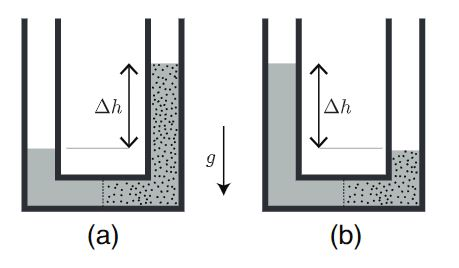
\includegraphics[height=5cm, width=6cm]{1.JPG}
    \end{center}

    \begin{enumerate}
      \item How many distinct orientations can the cube have?

        \textcolor{hwColor}{
          \\
          Considering each side of rthe cube an orientation, this cube has 6 distinct orientations. 
          (it has 6 faces and three different colors werer used)
          \\
        }

      \item 1 mole of such cubes are neatly stacked face-to-face into a large $3D$ cubic array, with each
      cube randomly aligned in one of its orientations. What is the entropy contribution arising
      from the orientational multiplicity of states?

        \textcolor{hwColor}{
          \\
          From page 75 of the textboom, we learned that the entropy of a system is defined as $S=k ~ ln \Omega$.
          Defining $N$ as the number of cubes we have:
          \\
          \\
          $
            S=k ~ ln 6^N \Longrightarrow \boxed{S=N k ~ ln 6} ~~~~ \checkmark
            \\
          $
        }

      \item What is the entropy contribution from orientations if the cube faces are all the same color?

        \textcolor{hwColor}{
          \\
          Well in case if all the cube faces are all the same color, then we have \emph{only} one orientation. Meaning,
          \\
          \\
          $
            S=k ~ ln 0 \Longrightarrow \boxed{S=0} ~~~~ \checkmark
            \\
          $
        }

    \end{enumerate}

    \pagebreak

    \item Estimate the work done by the diatomic gas in the cycle $ABCD$ in the below $PV$ diagram.

    \begin{center}
      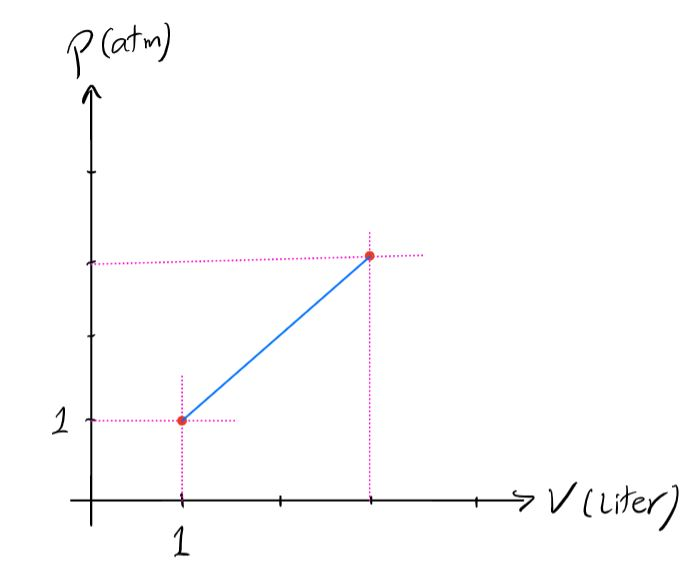
\includegraphics[height=8cm, width=10cm]{2.JPG}
    \end{center}

      \textcolor{hwColor}{
        \\
        $
          W=-\bigints\limits_{V_i}^{V_f} ~ P(V) dV
          \\
          \\
        $
        Note that for $AB$ and $CD$ the volume is constant and for $AD$ and $BC$ the pressure is constant.
        The work done for a gas is positive when volume is decreasing and it is negative when volume
        is increasing. Also, note that clockwise work done is positive and counter clockwise is negative.
        \\
        \\
        $
          \boxed{1 ~ bar=10^5 ~ pa}
          \\
          \\
          W=W_{BC}+W_{CD}+W_{DA}+W_{AB}
          \\
          \\
          \begin{cases}
            W_{BC}=\bigg( 10^5 ~ pa \bigg) \bigg( 3 ~ m^3 -2 ~ m^3\bigg)=2 \times 10^5
            \\
            \\
            W_{CD}=0
            \\
            \\
            W_{DA}=\bigg( 3 \times 10^5 \bigg) \bigg( 1 ~ m^3 - 3 ~ m^3 \bigg)=-6 \times 10^5
            \\
            \\
            W_{AB}=0
          \end{cases} \Longrightarrow W=2 \times 10^5+0-6 \times 10^5+0
          \\
          \\
          \\
          \therefore ~~~ \boxed{W=-400 ~ kJ}
        $
      }

  \end{enumerate}

\end{document}
